\documentclass[fleqn]{article}
\oddsidemargin 0.0in
\textwidth 6.0in
\thispagestyle{empty}
\usepackage{import}
\usepackage{amsmath}
\usepackage{graphicx}
\usepackage{flexisym}
\usepackage{calligra}
\usepackage{amssymb}
\usepackage{bigints} 
\usepackage[english]{babel}
\usepackage[utf8x]{inputenc}
\usepackage{float}
\usepackage[colorinlistoftodos]{todonotes}


\DeclareMathAlphabet{\mathcalligra}{T1}{calligra}{m}{n}
\DeclareFontShape{T1}{calligra}{m}{n}{<->s*[2.2]callig15}{}
\newcommand{\scriptr}{\mathcalligra{r}\,}
\newcommand{\boldscriptr}{\pmb{\mathcalligra{r}}\,}

\definecolor{hwColor}{HTML}{531C55}

\begin{document}

  \begin{titlepage}

    \newcommand{\HRule}{\rule{\linewidth}{0.5mm}}

    \center

    \begin{center}
      
\includegraphics[height=11cm, width=11cm]{asu.png}
    \end{center}

    \vline

    \textsc{\LARGE Classical Parts/Field/Matter II}\\[1.5cm]

    \HRule \\[0.5cm]
    { \huge \bfseries Problem Set 3}\\[0.4cm] 
    \HRule \\[1.0cm]

    \textbf{Behnam Amiri}

    \bigbreak

    \textbf{Prof: Maulik Parikh}

    \bigbreak

    \textbf{{\large \today}\\[2cm]}

    \vfill

  \end{titlepage}

  \begin{enumerate}
    \item The electric dipole moment of a single water molecule is about $6 \times 10^{-30}$ coulomb-meters. Imagine that all
    the molecular dipoles in a cup of water could be made to point down. Calculate the magnitude of the resulting surface charge 
    density at the upper surface of the water. How many electrons per square centimeter does that correspond to?

      \textcolor{hwColor}{
        \\
        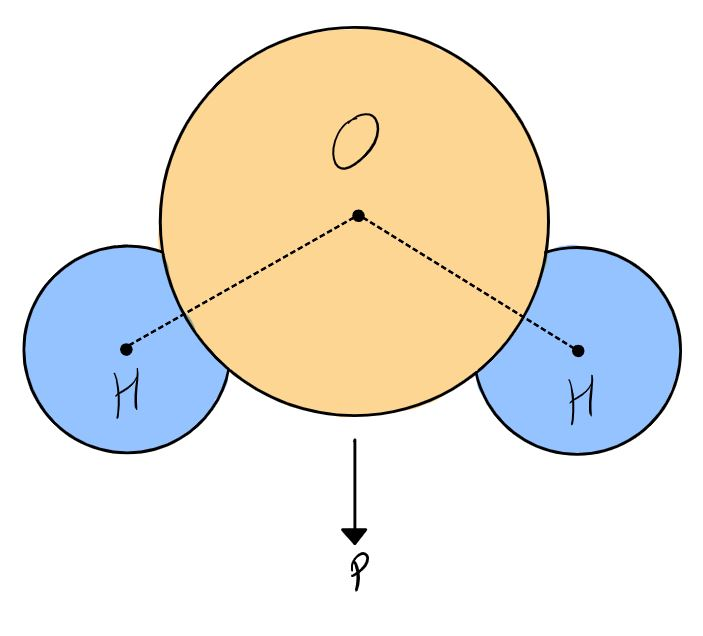
\includegraphics[height=5cm, width=6cm]{1.JPG}
        \\
        The dipole moment arises because oxygen is more electronegative than hydrogen; the oxygen pulls in the shared electrons 
        and increases the electron density around itself.The asymmetry of the water molecule leads to a dipole moment in the symmetry 
        plane pointed toward the more positive hydrogen atoms. The measured magnitude of this dipole moment is
        $$
          p=6 \times 10^{-30} ~ C.m 
        $$
        By consulting the Periodic Table of elements we get that water has a molecular weight of $18$ grams per mole. 
        We can convert moles to number of molecules by multiplying by Avogadro’s number.
        \\
        \\
        $
          n=\dfrac{1}{18} \times 6.02 \times 10^{23} \approx 3.33 \times 10^{22} ~~ \text{molecules per $cm^{-3}$}
        $
        \\
        \\
        We are told that the dipoles are all point down, therefore the polarization density is:
        \\
        \\
        $
          P=np=\left(
            3.33 \times 10^{22} ~~ \text{molecules per $cm^{-3}$}
          \right) \times 
          \left(
            6 \times 10^{-30} ~ C.m 
          \right)
          \\
          \\
          =\left(
            3.33 \times 10^{22} ~~ \text{molecules per $cm^{-3}$}
          \right) \times 
          \left(
            6 \times 10^{-28} ~ C.cm 
          \right)
          \\
          \\
          \\
          \therefore ~~~ P=1.998 \times 10^{-5} ~~~ C/cm^2 ~~~~ \checkmark
        $
        \\
        \\
        What we have now is the surface charge density $\sigma$. The number of electrons per square centimeter is:
        \\
        \\
        $
          \dfrac{\sigma}{e}=\dfrac{1.998 \times 10^{-5} ~~~ C/cm^2}{1.60 \times 10^{-19} ~~~ C}
          \\
          \\
          \\
          \therefore ~~~ \dfrac{\sigma}{e}=1.24875 \times 10^{14} ~~~ cm^{-2} ~~~~ \checkmark
        $ 
      }

    \item An electric dipole $\overrightarrow{p}$ is at the origin, at one corner of an equilateral triangle of side a, pointing 
    along one side (which you can take to be along the $\hat{+z}$ direction). A positive test charge qis initially at the corner at 
    the other end of that side (i.e. at $z=a$). Calculate the work done in moving the charge to the third corner of the triangle.

      % \textcolor{hwColor}{
      %   \\
      % }

    \item Consider a parallel-plate capacitor for which the plates are separated by a vertical distance $2d$. Suppose that the 
    space between the plates is filled with two slabs of linear dielectrics, each of thickness $d$. The upper slab has dielectric 
    constant $3$ and the lower slab has dielectric constant $2$. If the free charge density on the upper and lower plate is
    $+\sigma$ and $-\sigma$ respectively, calculate for each slab
    \begin{enumerate}
      \item The electric displacement.

        % \textcolor{hwColor}{
        %   \\
        % }

      \item The electric field.

        % \textcolor{hwColor}{
        %   \\
        % }

      \item The polarization.

        % \textcolor{hwColor}{
        %   \\
        % }

      \item The location and value of the bound charges.

        % \textcolor{hwColor}{
        %   \\
        % }
  
    \end{enumerate}

    \item A particle of charge qand rest mass mis moving with velocity $\overrightarrow{v}$ in a region where there 
    is a uniform magnetic field $\overrightarrow{B}$ perpendicular to $\overrightarrow{v}$. The Lorentz force causes 
    the particle to move in a circular path. Find the time required to complete one revolution. Specifically, consider
    a proton moving at a speed of $10,000 ~ km/s$ (which is still far slower than the speed of light, so ignore relativistic 
    effects) through a perpendicular interstellar magnetic field of strength $10^{-9} T$. Find the orbital time for the proton.

      % \textcolor{hwColor}{
      %   \\
      % }

    \item A cube of side $L$, centered at the origin, is made of a dielectric with a polarization $\overrightarrow{P}=k \overrightarrow{r}$.
    Find the bound charges and check that they add up to zero.

      % \textcolor{hwColor}{
      %   \\
      % }
  
    \item Three capacitors have identical area and plate separation. To be definite, let the plate separation direction be 
    the z-direction, and suppose the plates are separated by a distance $d$. Suppose one of the capacitors has only vacuum between the plates. The other two capacitors are
    each half-filled with a linear dielectric material, with dielectric constant $k$. In one of these, the dielectric material is 
    spread across all of one plate but extends only halfway to the other plate (i.e. to $d/2$ in the z-direction). In the other 
    capacitor, the same volume of dielectric material is present but arranged differently, covering only half the plate
    but extending all the way to the other plate. If the vacuum capacitor has a capacitance of C0, find the capacitance of each 
    of the other capacitors.

      % \textcolor{hwColor}{
      %   \\
      % }

  \end{enumerate}

\end{document}
